\documentclass[border=3pt]{standalone}
\usepackage{tikz}
\usetikzlibrary{arrows.meta,calc,positioning}
\tikzset{pin/.style={-{Stealth[length=5pt]}, thick},
  blk/.style={draw, thick, font=\sffamily\small, align=center}}
\begin{document}
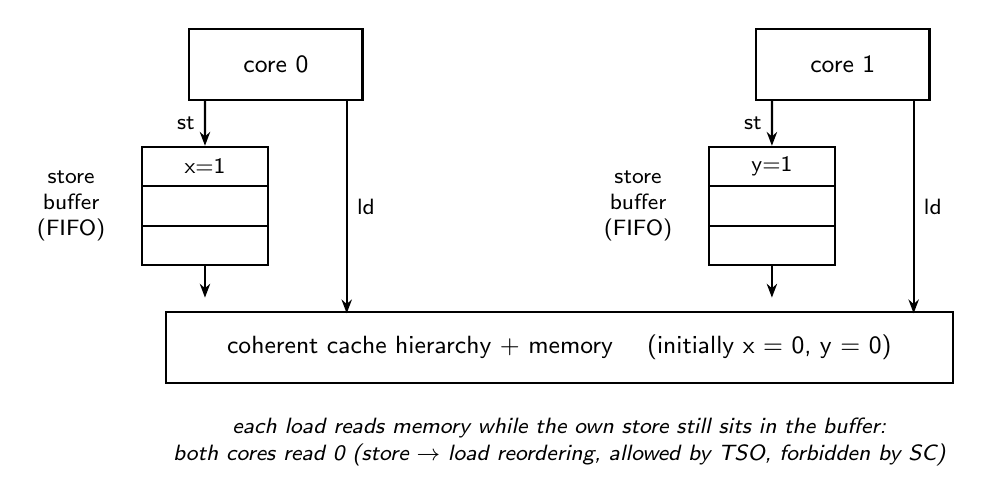
\begin{tikzpicture}[font=\sffamily\small]
  \foreach \i/\x/\st in {0/0/{x=1}, 1/7.2/{y=1}}{
    \node[blk, minimum width=22mm, minimum height=9mm] (c\i) at (\x,3.2) {core \i};
    % store buffer: 3 stacked slots
    \node[blk, minimum width=16mm, minimum height=5mm, font=\sffamily\footnotesize] (sb\i t) at (\x-0.9,1.9) {\st};
    \node[blk, minimum width=16mm, minimum height=5mm] (sb\i m) at (\x-0.9,1.4) {};
    \node[blk, minimum width=16mm, minimum height=5mm] (sb\i b) at (\x-0.9,0.9) {};
    \node[font=\sffamily\footnotesize, align=center] at (\x-2.6,1.4) {store\\buffer\\(FIFO)};
    \draw[pin] ($(c\i.south)+(-9mm,0)$) -- node[left, font=\sffamily\footnotesize]{st} (sb\i t.north);
    \draw[pin] (sb\i b.south) -- ++(0,-4mm);
    % load path bypasses the buffer
    \draw[pin] ($(c\i.south)+(9mm,0)$) -- node[right, font=\sffamily\footnotesize]{ld} ++(0,-27mm);
  }
  \node[blk, minimum width=100mm, minimum height=9mm] (mem) at (3.6,-0.4) {coherent cache hierarchy + memory \quad (initially x = 0, y = 0)};
  \node[font=\sffamily\footnotesize\itshape, align=center] at (3.6,-1.6) {each load reads memory while the own store still sits in the buffer:\\both cores read 0 (store $\rightarrow$ load reordering, allowed by TSO, forbidden by SC)};
\end{tikzpicture}
\end{document}
